\chapter[Computational Model]{Computational Model}
\label{chap:computational_model}

\lettrine{C}{alculating} changes to be performed based on user behavior is the challenge in question of this chapter.
The model presented here suggests a computational description of the convergence (or divergence) phenomenon, which aims to match the process the phonetic internal representation undergoes during a conversation.

\pagebreak

\section{From HHI to HCI}
\label{sec:from_hhi_to_hci}

Close examination of the results of the experiment described in \cref{sec:convergence_to_natural_and_synthetic_stimuli} revealed great variation across participants. \todo{take the slides that Iona prepared to show some differences either here or at the mentioned section}
While this is expected, it is worth looking into the nature of these variations, in order to spot the main influences on the convergence process.

\todo{is this a good place to mention and explain the human and machine metaphors?}
Since behavioral changes, e.g., as explained by \ac{cat}, happen naturally in \ac{hhi} and typically unawarely, it is not trivial to transfer them to computers, which need rules and some numeric representation to process.
Numeric representation can be achieved by applying some measuring technique appropriate for each feature (e.g., formant values for vowel quality).
Rules of different behaviors, however, cannot be directly constructed, due to the nature of this natural phenomenon, and can only be inferred from observed \ac{hhi} data.
The connecting link between the measured raw values and systematic rules is a machine-accessible representation of the convergence process.
Such representation would need to model, for example, the way humans percept the convergence-prone sounds, how they interact with previous instances and the current mental representation of the sound in question, and the cognitive process of the the phonetic changes.
Therefore, such a model should include the perception of the phonetic features, representation of the change in mental state of each feature in memory, and the realization of the changes during a conversation.
As these parts of the process are, by their nature, dependent on each other, the computational model presented here captures them as a linear pipeline (see \cref{sec:pipeline_representation}).

\section{Pipeline representation}
\label{sec:pipeline_representation}

As convergence happens automatically and seamlessly in human interlocutors' cognition, it is hard to say what are the exact steps this process comprises.
Merely observing convergence in \ac{hhi} does not shed any light on the internal process of changing the mental representation of features.
However, some key properties stand out when examining many occurrences in different interactions.
The pipeline representation presented here aims to capture these properties and offer a defined process of describing the changes (\crefrange{subsec:detect}{subsec:assign}).
The advantages of representing this process as a pipeline (as opposed to, e.g., a one-step, end-to-end conversion) is that each part in the process can be explained (and implemented, see \cref{subsec:computational_model,fig:adaptation_module_pipeline}) separately.
This enables combining different methods and implementations while keeping the steps independent of each other.
Therefore, only the \emph{order} of execution is important, which does not introduces any limitation, since it is expected to be -- and should be -- consistent.
This also allows performing specific steps in other, non-computational manners, like statistical-based (see \cref{chap:statistical_model}), \ac{ml}, or \ac{dl}.
Substituting specific steps gives the scientific freedom of experimenting with different methods without losing the core understanding of the convergence process and the ability to explain the meaning and contribution of each step.
For example, substituting the calculation method in the \textit{update} step or replacing it with a statistical-based method will of course influence the output of this step, but will not alter the role of it or influence the overall logic of the pipeline.

Note that although only phonetic convergence is discussed here, this pipeline could be used for describing changes in other type of features or modalities, like lexical choices, text complexity, or information density.
\review{need an abbreviation for information density?}
\review{need general references for these examples to give an idea what they are?}
This would naturally require some modifications\ldots

The proposed pipeline representation consists of five main steps: \emph{detect}, \emph{filter}, \emph{collect}, \emph{update}, and \emph{assign}.

\subsection{Detect}
\label{subsec:detect}

For changes on any level to happen, some feature that is prone to changes needs to be defined and occur in the speech input.
If these feature are not omitted in the interlocutors' speech, they are not likely to converge with regard to them, and will probably not register these changes as different realizations of these features.
Moreover, for the changes to register as a variation, the realization produced by the speaker must be prominent and distinctive enough to be perceived by the listener.

Which features fulfill this requirement is of course language- and culture-dependent, and might also differ based on the specific situation in which the interaction takes place.
For example, a feature of a language where a vowel can be alternatively realized by two different vowels will probably be ignored by a speaker of a language where only one of these vowels exist in its repository.
%Another option is that the additional vowel will cause confusion to the listener.
In this case, the two vowels will simply be mentally merged into one, causing no difficulties in comprehension, or as two completely different sounds in the language, as opposed to variations of the same sound that might potentially create confusion if another word is registered by the listener.

The input for this first step in the pipeline is the raw speech signal of the speaker, and its output is a list of phones representing phonemes that may trigger a phonetic change.
The \ac{asr} component of the system is responsible for detecting the phones realizations of phonemes that are defined as targets.
\putref{link to an example of feature definition}
These detected phones are then filtered in the \textit{Filter} step.

\subsection{Filter}
\label{subsec:filter}

The input for this step is the list of detected realizations of the defined target phonemes. After applying a filtering mechanism, it passes on only those phones from the list that occur in a change-prone position.
A target phoneme is a phoneme that serves as an anchor for a rule that aims to capture a phonetic feature or a more evolved phonological rule.
For example, the German phonological rule of \textipa{[@]} elision at words ending with \emph{-en} described in \cpageref{eq:shcwa_elision_rule} can be captured by the phoneme sequence /C\textipa{@n}/, where C represents a consonant (although in practice only a subset of the German consonants can be replaced by it in this context).
The anchor phoneme is \textipa{[@]} itself, since this is the segment that is subject to the change, namely the length -- or complete absence -- of it.
For this phenomenon, the target phoneme would be \textipa{@} and the measured feature would be segment length.
Another target feature described in \cref{subsec:target_features_HCIConv} is \textipa{[e:]} vs.\ \textipa{[E:]} realization of the mid-word grapheme \emph{ä}, which is captured by the target anchor phoneme \textipa{[E]} in a non-final position of a word.
Any defined feature goes through two filters. First, it required context to be an instance of the desired phonological phenomenon (C\textipa{@n} and non-final position for the above-mentioned features);
and secondly the defined accepted value range that would make it an acceptable instance of that phenomenon (for example, \textipa{[@]} length between \SI{0}{\milli\second} and \SI{60}{\milli\second} and appropriate F$_1$ and F$_2$ values for the \textipa{[e:]} and \textipa{[E:]} vowels in the above-mentioned features).
After applying these two filters, only those instances that truthfully capture the desired phonetic phenomenon are kept.

It is important to emphasize that this step is where phonetic expertise can be applied, both by defining the appropriate phonetic context of a feature, and by deciding on the appropriate values that should be considered for it.
For example, \textit{[@]} length of \SI{60}{\milli\second} can considered somewhat or disproportionately long in different situations. 

\subsection{Collect}
\label{subsec:collect}

After an instance of a feature was detected and validated in the filtering step, it needs to be registered as an exemplar of the feature it is associated with.
This stands in parallel to the way such exemplars (and in other contexts also words, meanings, etc.) are mentally stored in the human's short and long term memories.
Even though this process occurs unawarely (similarly to Exemplar Theory
\review{reference}
), but influences the way linguistic conventions and features of the language are represented -- and, by extension, produced -- by the speaker.
One of the complexities of modeling such internal representation is the interleaving influences of both long-term and short-term memory.
As this pipeline aims to describe convergence occurring within the scope of a single, isolated interaction (even if a long one), only short-term storage of exemplars is explicitly addressed in it.
The implementation of the implicit accounts of short-term and long-term memories representation is detailed in \cref{subsubsec:collecting_exemplars}.

To represent short-term memory of feature exemplars, a model must define how new exemplars are added, stored, retrieved and used (more in \cref{subsec:update}, and forgotten.
\cref{fig:exemplar_pool} gives a schematic overview of such model.
An exemplar is represented by a vector, where each dimension stands for a property of it based on the feature it is associated with (e.g., formant values for vowel quality features, pitch changes for intonation-related features, etc.).
Each feature has an \emph{exemplar pool}, containing the newly encountered exemplars.
This pool structured as a queue and represents the short-term memory of this feature.
New exemplars are \enquote{memorized}, i.e., added to the feature's pool.
The size of the pool can be defined by a parameter (see \cref{sec:parameters}).
If the pool is already at full capacity when a new exemplar is added, the oldest exemplar will be \enquote{forgotten}, i.e., deleted from the feature's pool.

This model of short-term memory of a feature's representation can be used to determine which exemplars are still affecting the speaker's mental representation of a feature, and therefore will be taken into account when it is produced.
Temporal aspects of the exemplars can be taken into account as well.
For example, the time interval between acquired exemplars can alter their degree of influence on the feature's state, or temporally close clusters of exemplars may have greater influence, etc.

\begin{figure}[t]
	\centering
	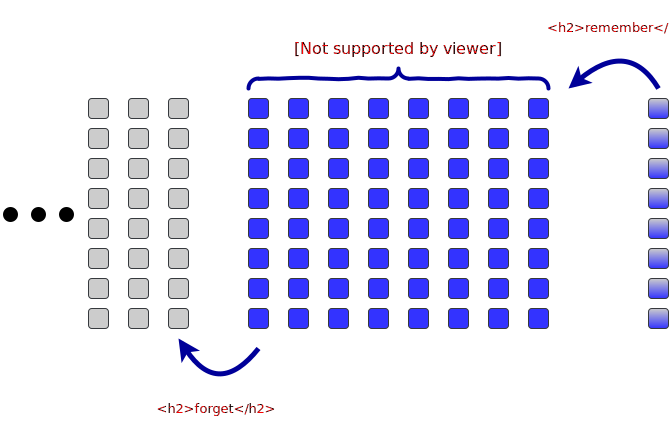
\includegraphics[width=\textwidth]{pool}
	\caption
	[The exemplar pool]
	{A new exemplar is added to the feature's pool when encountered.
		Old exemplars are removed when the pool is full.
		Exemplars currently in the pool are taken into account when the realization of the feature is determined.
		Each dimension of an exemplar represents a property of the feature it is associated with.}
	\label{fig:exemplar_pool}
\end{figure}

\subsection{Update}
\label{subsec:update}

The core of the convergence process is the change itself in feature mental state.
As describe above, the \textit{collect} step is responsible for storing new feature exemplars and forgetting older ones.
This step is responsible for how these stored exemplars are actually handled, the relations and hierarchies between them, and ultimately the convergence effect itself.
Each feature has a state, which is the model's corresponding of a human's current mental representation of this feature.
This state is used whenever the value of this feature is needed, e.g., in the \textit{assign} step (see \cref{subsec:assign}).
However, the change of this state is determined in the \textit{update} step.
More precisely, a new state will be generated every time this step is triggered, based on the current state and the exemplars in the pool.
A trigger might be exemplar-based, i.e., after a certain number of new exemplars were added, or time-based, i.e., every time a pre-determined amount of time had passed.
\todo{example/motivation for each}
\todo{calculation methods}

\subsection{Assign}
\label{subsec:assign}

\todo[inline]{explain the limitation mechanism and why it's needed}

\begin{figure}
	\centering
	\includegraphics[width=\textwidth]{synthesis}
	\caption
	[Manipulated features on a synthesized waveform]
	{An illustration of a manipulated output audio waveform.
		Each colored pin marks a phonetic features captured and processed by the pipeline.}
	\label{fig:adapted_synthesis_output}
\end{figure}

\section{Parameters}
\label{sec:parameters}

To allow degrees of freedom within the computational model described in \cref{chap:computational_model}, some parameters need to be introduced.
These parameters are the connecting link between the theoretical, schematic model and the implementation of the module as part of an \acs{sds} (see \cref{chap:convergence_module_for_sdss}).
They are also the key for experimentation with the model in various scenarios on the look for the best configurations in different situations.

As shown in \cref{sec:convergence_to_natural_and_synthetic_stimuli}, not all participant showed the same \textit{sensitivity} toward changes in the stimuli in general.
Here sensitivity refers to the degree of adaptation toward a stimulus.
In addition, when one does converge, the sensitivity to changes (i.e.~the \enquote{amount of differentiation}) toward a single stimulus might differ.
In the model, these two aspects were combined into one parameter -- \textit{convergence rate}.
\todo{write a sentence that this rate is a balance between current and new style. put equation}
For simulating the case where a participant does not converge at all, this rate can be set to zero.
In that case the model will ignore the other interlocutor's speech and stick to the current speech style.
Another variation found among the participants was the overall convergence degree toward the stimuli.
In other words, where would the convergence process stop.
This is simulated by the parameters \textit{convergence limit}, which defines the maximally allowed degree of similarity between the interlocutors.
The value of this parameter is between zero and one.
When set to 1.0 (\SI{100}{\percent}), the model is allowed to change up to \SI{100}{\percent} toward the other interlocutor; when set to 0.8, up to \SI{80}{\percent}, and so on.
The parameter is used to control that the model does not simply imitate the user's input, which might happen especially with high convergence rate.
By limiting the change, the convergence process is more gradual and restrained.

However, parameters simulating the actual change are not enough.
To properly model an interlocutor, some individual aspect that are not directly related to the speech output are required as well.

The convergence target depends on the recent instances of the variable feature (or \textit{exemplars}).
How many exemplars are taken into account when the feature's mental representation is updated depends on the interlocutor's short memory capacity.
Working memory is a complex mechanism
\review{reference for modeling working memory?}
.
It is modeled in a very simplified manner here, namely by the number of exemplars the interlocutor currently remembers on a first-in-first-out basis, i.e.~the \textit{exemplar pool size}.
An exemplar is modeled as a vector with cardinality $n$, where $n$ is the number of dimensions the feature has (e.g.~the number of measured formants for a vowel-quality feature).
Whenever an instance of the feature is encountered, a new exemplar is added to the pool.
If the pool is already in full capacity, the oldest exemplar is forgotten by the speaker (deleted in the model) (see \cref{fig:exemplar_pool}).

Individuals may also have different general \textit{tendency} to converge toward other interlocutors.
Here tendency refers to the likelihood to adapt to the stimuli presented to them.
This likelihood is modeled not probabilistically, but by an \textit{update frequency}.
After an exemplar is added to a feature's pool, an update of the feature's value may be triggered.
Whether and how often this happens is determined by the \textit{update frequency}.
If set to 1, an update will occur every time an exemplar is added; if set to 2, every other exemplar, and so on.
When set to 0, however, updates will only take place when explicitly requested.
This can be useful when, for example, all features are to be updated at the same time, regardless of how many exemplars have been accumulated for each feature.
Increasing the update interval means that each new pool value will be affected by more new exemplars, which, depending on the calculation method used (see below), might result in a smoother converging process.
Additionally, a longer update interval also means that convergence will generally take longer, since the model's features are not being updated as frequently.

Though not only the frequency in which the update occurs plays a roll in the process, but also the manner in which it is being updated.
This manner is determined by the \textit{calculation method} used.
Since the features in the model are represented by vectors, any function that takes a vector as input and outputs another as output would do.
\todo{explain that first we need to transform the matrix!}

After transforming the matrix, the model has a representation of each feature as a vector where each dimension is a single value of a 
One option is to use a fixed function on each of the dimensions to create a vector with new values.
This function could be, for example, simple average or decaying average.
Such functions are easy to understand and follow, and can describe relatively simple mechanics of how each stimulus contributes to the overall change, since each value is calculated sequentially but independently of the other.

Each feature can use a different calculation method.
Which method to use is up to the user of the system, as there might be acoustic or psycholinguistic constrains to take into account, based on the settings the system is used in (experimental, exploratory, data collection, etc.)

% calculation method -- make sure you directly lead to it from the update step

\todo{put equations where appropriate}

\begin{landscape}
	\begin{table}[tb]
		\centering
		\caption[Summary of computational model's parameters]{Computational model's parameters in their order of use.}
		\label{tab:comp_model_parameters}
		\begin{tabulary}{\linewidth}{lLL}
			\toprule
			\multicolumn{1}{c}{\textbf{Parameter}} 		& \multicolumn{1}{c}{\textbf{Description}} 					& \multicolumn{1}{c}{\textbf{Value}} \\
			\textit{target phoneme*} 					& the phoneme that triggers the feature 					& phoneme symbol\\
			\textit{phonetic context*} 					& the environment in which the phoneme is accepted 			& regex of phoneme symbols\\
			\textit{allowed range*} 					& the value range in which new instances are accepted 		& numeric, depending on feature\\
			\textit{exemplar pool size} 				& maximum number of exemplars in memory 					& integer, $> 0$\\
			\textit{update frequency} 					& how frequently a feature's value is recalculated 			& integer, $\geq 0$ \\
			\textit{calculation method*} 				& the manner in which the pool value is calculated 			& one of supported methods\\
			\textit{convergence rate} 					& weight given to the pool value 							& float, typically $> 0$ and $< 1$\\
			\textit{convergence limit*}  				& the maximum degree of convergence allowed for a feature 	& float, $> 0$ and $< 1$ \\	
			\bottomrule
		\end{tabulary}
		\flushleft{\footnotesize \emph{* denotes parameters that are defined individually for each feature}}
	\end{table}
\end{landscape}


The model's parameters are summarized in \cref{tab:comp_model_parameters}
With these criteria in mind, a computational model with several parameters wad developed.
This model, described in detail in \citet{Raveh2017Interspeech}, includes these parameters and a few others, and its purpose is to generate different convergence behaviors.

% briefly also mention target phoneme and phonetic context
